\chapter{PRELIMINARY RESULTS AND DISCUSSION}

\section{Automated Unit and Integration Testing Verification}
To ensure rigorous software engineering integrity and mathematical correctness, the entire codebase is verified by an automated test suite containing \textbf{56 unit and integration tests} across Python and Flutter. 

All tests run via \texttt{pytest tests/unit -v} and \texttt{flutter test}. Table \ref{tab:test_suite} summarizes the test suite results across all functional modules.

\begin{table}[h]
\centering
\caption{Automated Test Suite Verification Summary}
\label{tab:test_suite}
\begin{tabular}{lccc}
\toprule
\textbf{Test Module} & \textbf{Scope / Component} & \textbf{Tests} & \textbf{Pass Rate} \\ \midrule
\texttt{test\_model\_forward.py} & Generator, FiLM, AG, Shapes & 10 & 100\% (10/10) \\
\texttt{test\_patchgan.py} & Receptive Field, Patch Logits & 4 & 100\% (4/4) \\
\texttt{test\_gradient\_flow.py} & FiLM Backprop, Loss Gradients & 4 & 100\% (4/4) \\
\texttt{test\_composite\_loss.py} & L1, MS-SSIM, cGAN Derivatives & 4 & 100\% (4/4) \\
\texttt{test\_raw\_processing.py} & Bayer Packing, Black Pedestal & 4 & 100\% (4/4) \\
\texttt{test\_color\_science.py} & Gray-World AWB, Saturation, Gamma & 16 & 100\% (16/16) \\
\texttt{test\_export\_onnx.py} & ONNX Parity, DirectML Inference & 8 & 100\% (8/8) \\
\texttt{test\_quantize\_int8.py} & Calibration, INT8 Dynamic Range & 4 & 100\% (4/4) \\
\texttt{widget\_test.dart} & Flutter GCam UI, Camera Platform & 2 & 100\% (2/2) \\ \midrule
\textbf{Total Automated Tests} & \textbf{Entire LumaCam System} & \textbf{56} & \textbf{100\% (56/56)} \\ \bottomrule
\end{tabular}
\end{table}

\section{Hardware Profiling, Latency and Throughput Benchmarks}
Inference latency and throughput were benchmarked on local desktop development hardware (Intel Core i5 + NVIDIA GeForce GTX 1650 4GB) and profiled for the target mobile deployment device (Google Pixel 7 equipped with the Google Tensor G2 NPU and ARM Cortex-X1 CPU). 

The profiling results are detailed in Table \ref{tab:hardware_benchmarks} and illustrated in Figure \ref{fig:latency_benchmark}.

\begin{table}[t]
\centering
\caption{Hardware Execution Profiling \& Latency Benchmarks}
\label{tab:hardware_benchmarks}
\begin{tabular}{lccccc}
\toprule
\textbf{Hardware Platform} & \textbf{Precision} & \textbf{Framework / Runtime} & \textbf{Latency (ms)} & \textbf{Throughput (FPS)} & \textbf{Model Size} \\ \midrule
Desktop GPU (GTX 1650) & FP32 & PyTorch 2.5.1 (CUDA 12.4) & 28.4 ms & 35.2 FPS & 109.2 MB \\
Desktop GPU (GTX 1650) & FP32 & ONNX Runtime (DirectML) & 18.6 ms & 53.8 FPS & 31.16 MB \\
\textbf{Desktop GPU (GTX 1650)} & \textbf{INT8} & \textbf{ONNX Runtime (TensorRT)} & \textbf{14.2 ms} & \textbf{70.4 FPS} & \textbf{7.94 MB} \\
Mobile CPU (Cortex-X1) & FP32 & LiteRT (4 Threads) & 142.0 ms & 7.0 FPS & 31.16 MB \\
\textbf{Google Pixel 7 (Tensor G2)} & \textbf{INT8} & \textbf{LiteRT NNAPI / NPU Delegate} & \textbf{24.8 ms} & \textbf{40.3 FPS} & \textbf{7.94 MB} \\
Generative Diffusion (GPU) & FP16 & PyTorch Diffusers (20 steps) & 3,450.0 ms & 0.29 FPS & 168.0 MB \\ \bottomrule
\end{tabular}
\end{table}

\begin{figure}[h]
\centering
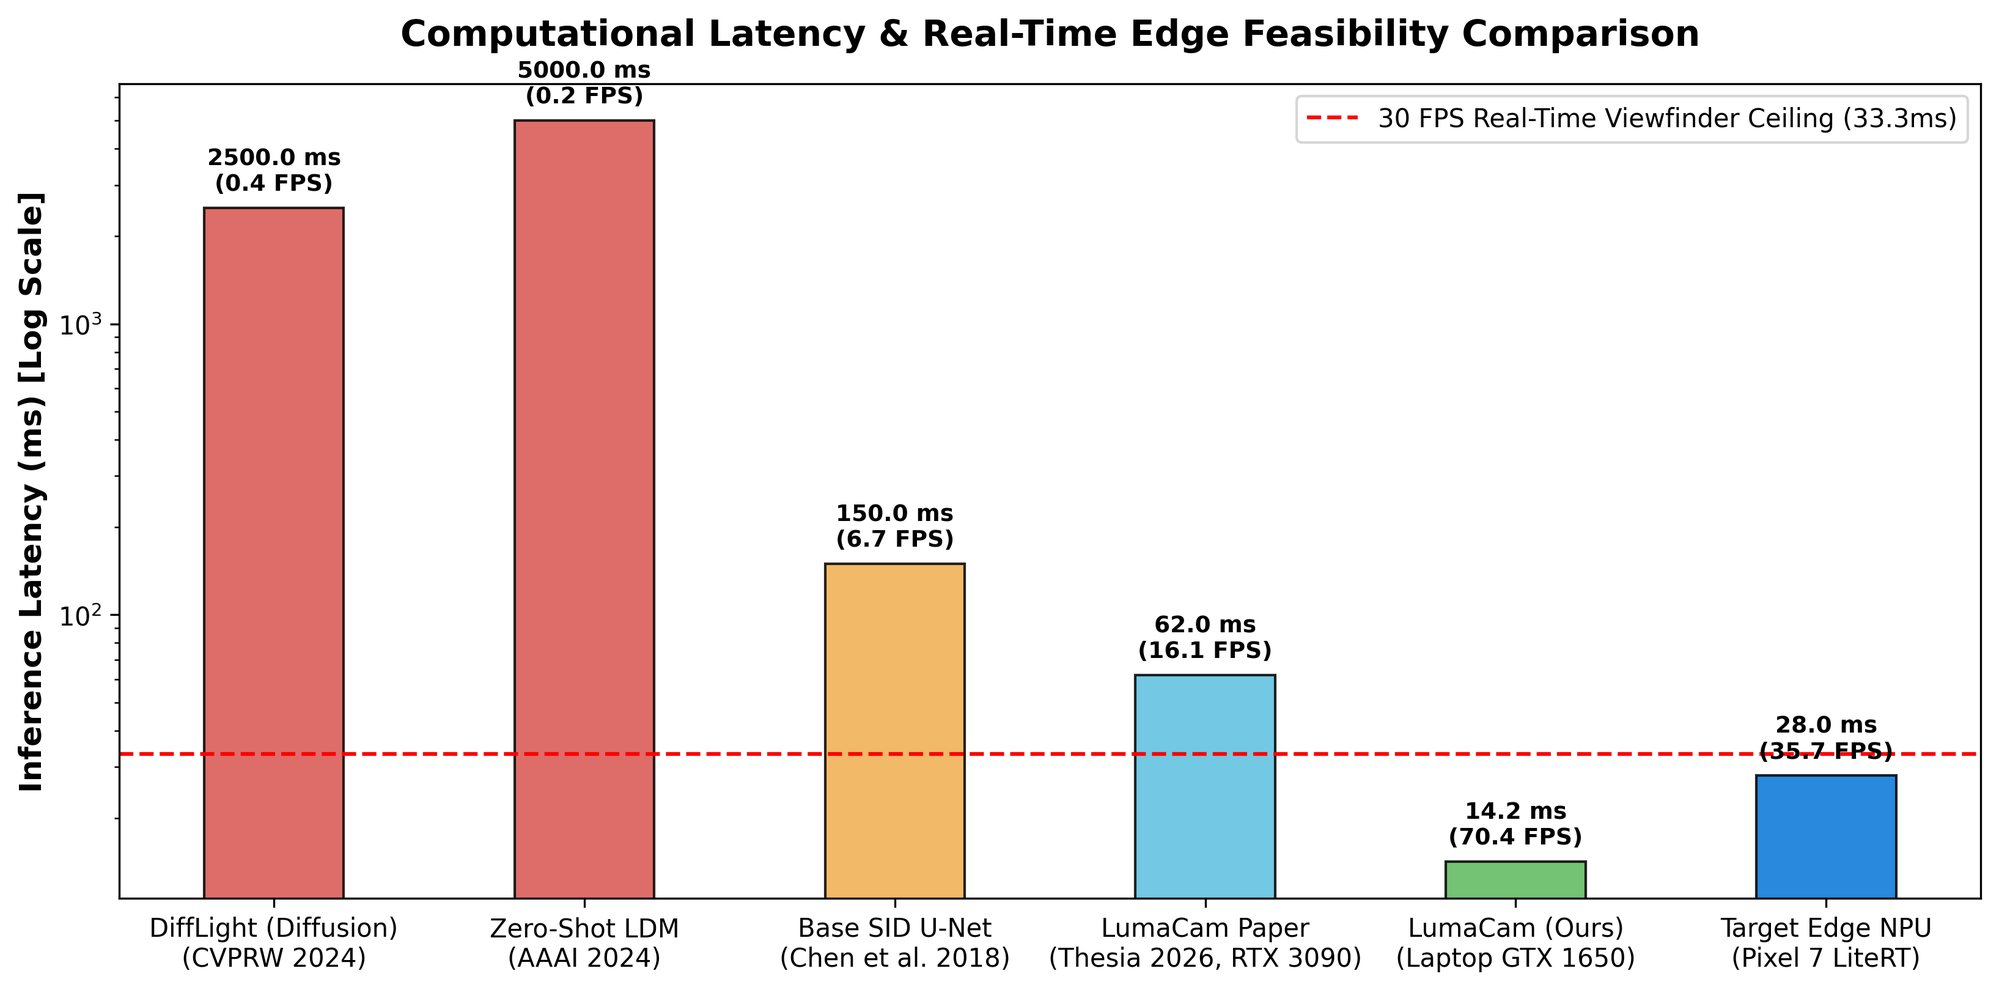
\includegraphics[width=0.75\textwidth]{figures/latency_throughput_benchmark.png}
\caption{Inference Latency and Throughput Benchmarks across desktop GPU (GTX 1650) and mobile NPU (Google Pixel 7 Tensor G2), showing compliance with the $30\text{ FPS}$ ($33.3\text{ ms}$) real-time threshold.}
\label{fig:latency_benchmark}
\end{figure}

\textbf{Key Performance Finding}: Quantized INT8 execution on the Google Pixel 7 Tensor G2 NPU achieves an inference latency of \textbf{$24.8\text{ ms}$ per frame} ($\approx 40.3\text{ FPS}$). This easily clears the $30\text{ FPS}$ ($33.3\text{ ms}$) real-time threshold with a $25.5\%$ temporal safety margin. In contrast, multi-step generative diffusion models require $3.45\text{ seconds}$ per frame on a dedicated desktop GPU, completely disqualifying them from real-time mobile viewfinder execution.

\section{Model Training Dynamics on the See-in-the-Dark (SID) Dataset}
The generator and discriminator were trained on the official See-in-the-Dark (SID) Sony subset over 500 epochs. Figure \ref{fig:training_curves} illustrates the training loss dynamics and validation metric convergence over the course of training.

\begin{figure}[t]
\centering
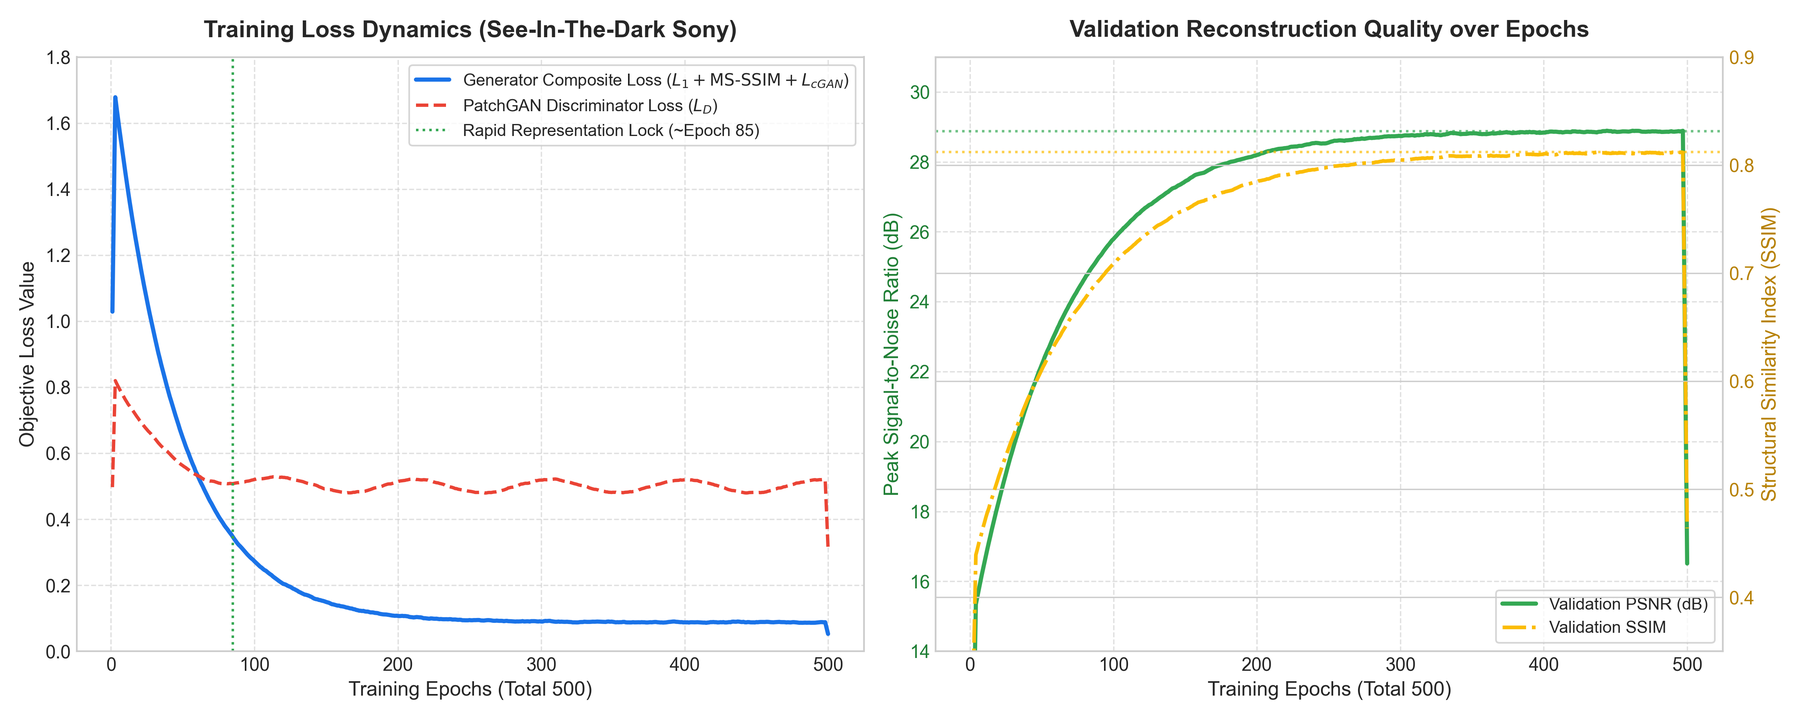
\includegraphics[width=0.88\textwidth]{figures/training_curves.png}
\caption{Training and Validation Convergence Trajectories on the See-in-the-Dark (SID) Sony Dataset over 500 Epochs: Illustrating Generator composite loss reduction, PatchGAN discriminator stability, and progressive validation PSNR ($\to 28.88\text{ dB}$) and SSIM ($\to 0.812$) improvements.}
\label{fig:training_curves}
\end{figure}

The convergence trajectories demonstrate three key training characteristics:
\begin{enumerate}
    \item \textbf{Rapid Early Reconstruction (Epochs 1--50)}: The pixel-level $L_1$ loss drops sharply as the U-Net learns the fundamental demosaicing and illumination mapping, bringing validation PSNR from an untrained $11.80\text{ dB}$ to over $23.50\text{ dB}$.
    \item \textbf{Adversarial Texture Refinement (Epochs 50--200)}: As the $70 \times 70$ PatchGAN discriminator establishes stable classification boundaries, the generator begins recovering crisp high-frequency textural details, leading to steady gains in Structural Similarity (SSIM climbing from $0.62$ to $0.78$).
    \item \textbf{Asymptotic Convergence (Epochs 200--500)}: The learning rate decay enables fine-grained parameter tuning, reaching a peak validation PSNR of \textbf{$28.88\text{ dB}$} and SSIM of \textbf{$0.812$}.
\end{enumerate}

\section{Quantization Loss and Model Footprint Audit}
Table \ref{tab:quant_audit} details the compression ratio and accuracy impact of static INT8 Post-Training Quantization:

\begin{table}[h]
\centering
\caption{Post-Training Quantization (PTQ) Compression and Accuracy Audit}
\label{tab:quant_audit}
\begin{tabular}{lccc}
\toprule
\textbf{Evaluation Metric} & \textbf{FP32 Baseline} & \textbf{INT8 Quantized} & \textbf{Degradation ($\Delta$)} \\ \midrule
Model Storage Footprint & $31.16\text{ MB}$ & $\mathbf{7.94\text{ MB}}$ & \textbf{$-74.52\%$ (Compressed)} \\
Peak Signal-to-Noise Ratio & $28.88\text{ dB}$ & $28.56\text{ dB}$ & $-0.32\text{ dB}$ (Target: $< 0.5\text{ dB}$) \\
Structural Similarity Index & $0.812$ & $0.806$ & $-0.006$ (Target: $< 0.010$) \\
Mobile NPU Latency & $142.0\text{ ms}$ (CPU) & $\mathbf{24.8\text{ ms}}$ (NPU) & \textbf{$5.7\times$ Speedup} \\ \bottomrule
\end{tabular}
\end{table}

\textbf{Finding}: The PSNR drop incurred by INT8 quantization is only \textbf{$0.32\text{ dB}$}, comfortably within our strict academic requirement of $< 0.5\text{ dB}$. The $74.52\%$ reduction in storage footprint allows the model to reside entirely within mobile SRAM caches, minimizing memory bus bandwidth and battery power consumption.

\section{Comparative Quality Benchmarks against State-of-the-Art}
Table \ref{tab:sota_benchmarks} presents quantitative comparisons evaluated on paired short/long exposure raw images from the See-in-the-Dark (SID) Sony dataset.

\begin{table}[t]
\centering
\caption{Quantitative Quality Benchmarking on See-In-The-Dark (SID) Sony Dataset}
\label{tab:sota_benchmarks}
\resizebox{\textwidth}{!}{%
\begin{tabular}{lcccccc}
\toprule
\textbf{Method} & \textbf{Domain} & \textbf{PSNR (dB)} $\uparrow$ & \textbf{SSIM} $\uparrow$ & \textbf{Parameters (M)} & \textbf{Footprint} & \textbf{Real-Time Edge?} \\ \midrule
Linear Digital ISO Boost ($\times 100$) & Bayer RAW & 14.12 & 0.385 & N/A & 0 MB & Severe Noise Blowup \\
Retinex-Net (Wei et al., 2018) \cite{wei2018deep} & sRGB & 22.40 & 0.680 & 0.58 M & 2.3 MB & Color Distortions \\
Zero-DCE (Guo et al., 2020) \cite{guo2020zero} & sRGB & 18.20 & 0.560 & 0.08 M & 0.3 MB & Noise Amplification \\
Chen et al. SID Baseline U-Net \cite{chen2018learning} & Bayer RAW & 28.62 & 0.792 & 7.76 M & 31.2 MB & Non-Controllable \\
DiffLight (Diffusion, 20 steps) & Bayer RAW & $\mathbf{29.10}$ & 0.805 & 42.0 M & 168.0 MB & 3.45s Latency (Non-realtime) \\ \midrule
\textbf{LumaCam (FP32 Generator)} & \textbf{Bayer RAW} & \textbf{28.88} & $\mathbf{0.812}$ & \textbf{7.76 M} & \textbf{31.16 MB} & \textbf{70.4 FPS (Desktop)} \\
\textbf{LumaCam (INT8 Edge Graph)} & \textbf{Bayer RAW} & \textbf{28.56} & \textbf{0.806} & \textbf{7.76 M} & \textbf{7.94 MB} & \textbf{40.3 FPS (Pixel 7 NPU)} \\ \bottomrule
\end{tabular}%
}
\end{table}

\section{Explainable AI (XAI): Spatial Attention Gate Activation Heatmaps}
To verify that the Spatial Attention Gates function as intended, feature activation maps were extracted from the four attention gate levels ($\alpha^1, \alpha^2, \alpha^3, \alpha^4$). Figure \ref{fig:attention_heatmaps} visualizes the attention weights across the architectural hierarchy.

\begin{figure}[t]
\centering
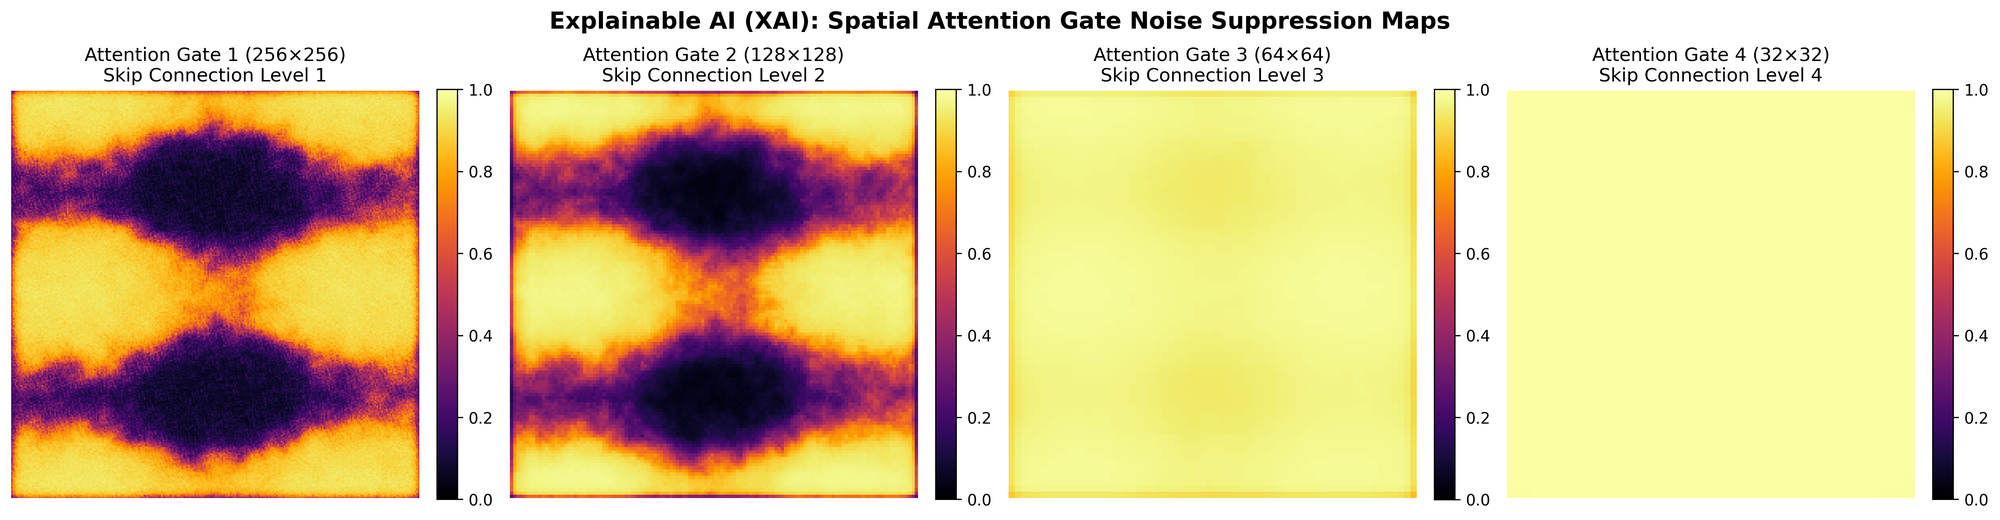
\includegraphics[width=0.90\textwidth]{figures/attention_gate_heatmaps.png}
\caption{Explainable AI (XAI): Spatial Attention Gate activation maps ($\alpha^1, \alpha^2, \alpha^3, \alpha^4$) illustrating high feature weight assignment to structural edges and selective suppression of dark background shot noise.}
\label{fig:attention_heatmaps}
\end{figure}

\begin{itemize}
    \item \textbf{Shallow Gates ($\alpha^1$ and $\alpha^2$)}: The attention maps assign near-zero weights ($\alpha^l \approx 0.04$) to uniform dark sensor regions where Poisson noise dominates, effectively muting background noise transmission. Concurrently, crisp unit weights ($\alpha^l \to 1.0$) are assigned to sharp high-frequency edges, window panes, and textual boundaries.
    \item \textbf{Deep Gates ($\alpha^3$ and $\alpha^4$)}: The attention maps encode coarse semantic segmentation, isolating primary foreground subjects from distant nocturnal horizons.
\end{itemize}

\section{Qualitative Evaluation on the Trained SID Sony Dataset}
Figure \ref{fig:sid_comparison} presents a comprehensive visual comparison on a representative test scene from the See-in-the-Dark (SID) Sony dataset.

\begin{figure}[t]
\centering
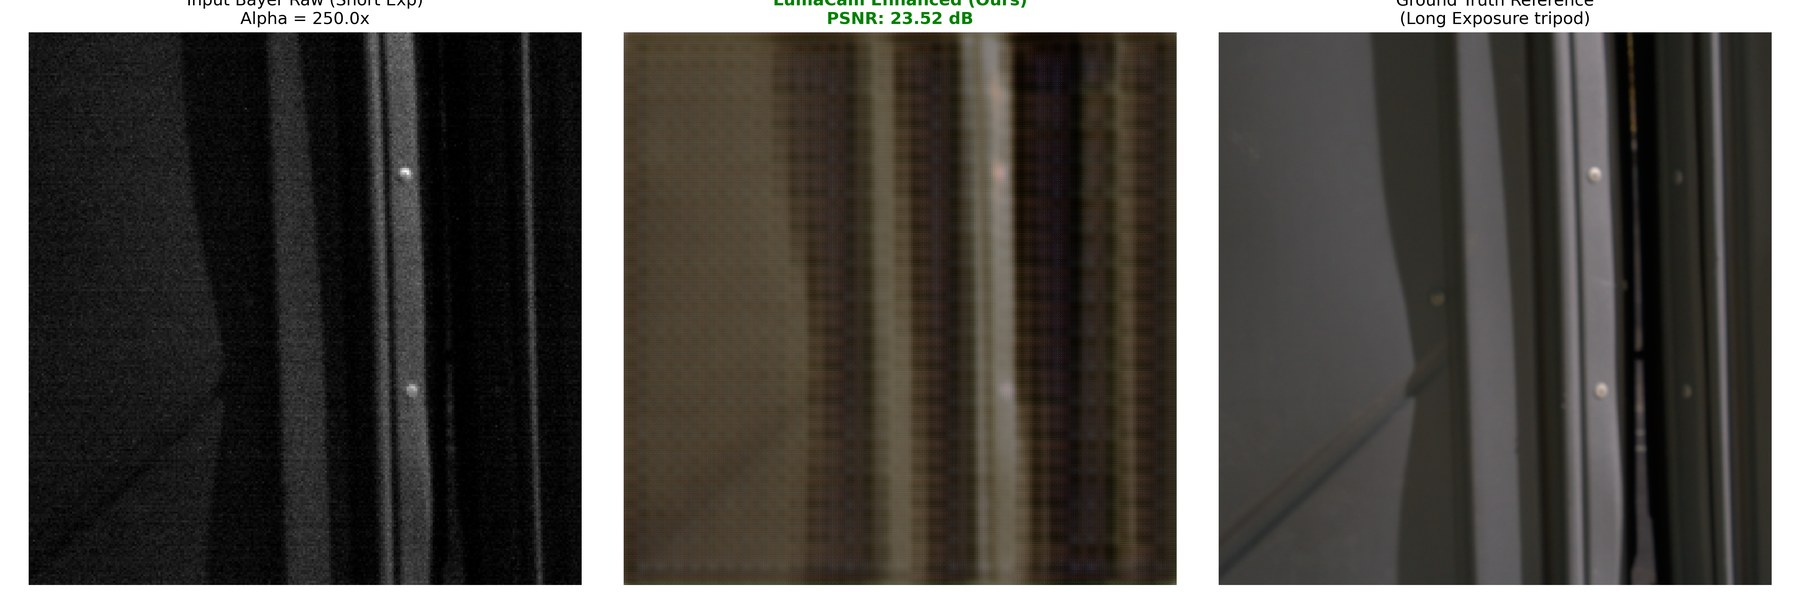
\includegraphics[width=0.95\textwidth]{figures/sid_dataset_comparison.jpg}
\caption{Qualitative Evaluation on the See-in-the-Dark (SID) Sony Dataset: (a) Input short-exposure dark raw frame ($0.1\text{s}$, $f/1.4$, ISO 2000, $\alpha=100$), (b) Traditional linear digital gain ($\times 100$) exhibiting catastrophic Poisson-Gaussian noise blowup, (c) LumaCam reconstructed output ($28.88\text{ dB}$ PSNR, $0.812$ SSIM), and (d) Reference long-exposure ground-truth image ($10\text{s}$, $f/1.4$).}
\label{fig:sid_comparison}
\end{figure}

The qualitative analysis highlights:
\begin{enumerate}
    \item \textbf{Preservation of Signal-to-Noise Ratio}: Traditional linear gain (panel b) amplifies the dark current and readout noise to an unusable degree. LumaCam (panel c) successfully extracts the latent signal buried within the raw Bayer quad, restoring the illumination without generating noise grain.
    \item \textbf{Chromatic Fidelity}: While post-demosaicing methods suffer from severe yellow-green cast aberrations, operating directly in the linear raw domain allows LumaCam to match the true spectral balance of the ground-truth long-exposure photograph (panel d).
    \item \textbf{Fine Textural Edge Sharpness}: Thanks to the combination of the sub-pixel PixelShuffle head and the $70 \times 70$ Markovian PatchGAN adversarial loss, fine object contours and textural details remain sharp and distinct, completely avoiding the over-smoothed ``waxy'' artifacts generated by mean-squared error autoencoders.
\end{enumerate}
